\documentclass[a4paper,12pt]{article}

\usepackage[utf8x]{inputenc}
\usepackage[english,hungarian]{babel}
\usepackage[margin=1in]{geometry}

\usepackage{indentfirst}
\usepackage{fancyhdr}
\pagestyle{fancy}

\usepackage[table,xcdraw,dvipsnames]{xcolor}
\definecolor{whitesmoke}{rgb}{0.96,0.96,0.96}
\definecolor{lightblue}{rgb}{0.22,0.45,0.70}
\definecolor{darkred}{rgb}{0.9,0.0,0.0}

\usepackage[backref=false,pagebackref=true]{hyperref}
\hypersetup{colorlinks=true,urlcolor=lightblue,citecolor=green!75!black,linkcolor=orange!98!black,pdfborder={0 0 0}}
\usepackage{multirow}

\usepackage{graphicx}
\usepackage{wrapfig}

\usepackage{booktabs}
\usepackage{multicol}
\usepackage{amsmath}

\usepackage{tikz}
\usetikzlibrary{arrows}
\tikzstyle{es} = [-triangle 60]

\usepackage{enumitem}
\setlist[itemize]{itemsep=0pt}
\setlist[enumerate]{itemsep=0pt}

\setlength{\parindent}{2em}
\setlength{\parskip}{0.25em}

\renewcommand{\arraystretch}{2}

\usepackage[T1]{fontenc}
\usepackage{lmodern}
\usepackage{fontawesome}

\newcommand{\urlprefix}{Forrás: \urlstyle{rm}}

\newcommand{\refspace}{\vspace{-2mm}}
\newcommand{\redarrow}{\textcolor{darkred}{$\mathbf{\to}$}}
\makeatletter
\def\BR@@bibitem#1#2\par{
	\let\backrefprint\BR@backrefprint
	\def\@linkcolor{black}
	\BRorg@bibitem{#1}#2\redarrow \thinspace \BR@backref{#1}
}
\makeatother

\usepackage{titlesec}
\titleclass{\subsubsubsection}{straight}[\subsection]

\newcounter{subsubsubsection}[subsubsection]
\renewcommand\thesubsubsubsection{\thesubsubsection.\arabic{subsubsubsection}}
\titleformat{\subsubsubsection}
  {\normalfont\normalsize\bfseries}{\thesubsubsubsection}{1em}{}
\titlespacing*{\subsubsubsection}
{0pt}{3.25ex plus 1ex minus .2ex}{1.5ex plus .2ex}

\makeatletter
\def\toclevel@subsubsubsection{4}
\def\l@subsubsubsection{\@dottedtocline{4}{7em}{4em}}
\makeatother

\setcounter{secnumdepth}{4}
\setcounter{tocdepth}{4}

\usepackage{minted}
\renewcommand{\theFancyVerbLine}{\rmfamily\scriptsize\arabic{FancyVerbLine}}
\setminted{linenos,autogobble,breaklines,fontsize=\footnotesize,tabsize=4,numbersep=7pt,bgcolor=whitesmoke}
\AtBeginEnvironment{minted}{\renewcommand{\fcolorbox}[4][]{#4}}

\author{Bogosi Roland}
\title{Behatolástesztelő és sebezhetőségfelderítő rendszer}

\begin{document}
\pagestyle{empty}
\selectlanguage{hungarian}

	\begin{center}
		{\Large Sapientia Erdélyi Magyar Tudományegyetem}\\\vspace{0.05in}
		{\Large Műszaki és Humántudományok Kar, Marosvásárhely}\\\vspace{0.07in}
		{\Large Számítástechnika}\\
		
		\vspace{2.5in}
		
		{\huge Behatolástesztelő és Sebezhetőségfelderítő}\\\vspace{0.1in}
		{\huge Rendszer}
		
		\vspace{0.5in}
		
		{\LARGE TDK Dolgozat}
		
	\end{center}
	
	\vspace{2.0in}
	
	\begin{multicols}{2}
		\begin{flushleft}
			{\Large Vezető tanár:}\\\vspace{0.1in}
			{\LARGE {Dr. Vajda Tamás}}
		\end{flushleft}
		\columnbreak
		\begin{flushright}
			{\Large Diák:}\\\vspace{0.1in}
			{\LARGE {Bogosi Roland}}
		\end{flushright}
	\end{multicols}
	
	\vspace{1.5in}
		
	\begin{center}
		{\LARGE 2016}
	\end{center}

\newpage
\section*{Tartalomjegyzék}

	\begingroup
	\renewcommand{\section}[2]{}
	\hypersetup{linkcolor=lightblue}
	\setlength{\parskip}{0em}
	\tableofcontents
	\endgroup

	\begingroup
	\hypersetup{linkcolor=lightblue}
	\listoffigures
	%\listoftables
	\renewcommand*{\listoflistingscaption}{Kódrészletek jegyzéke}
	\listoflistings
	\endgroup

\newpage
\pagestyle{fancy}
\section{Projekt Célja}

	A projekt célja egy olyan alkalmazás fejlesztése amely egy bizonyos hálózatot fel tud térképezni és a rajta található sebezhetőségeket fel tudja deríteni.
	
	Az alkalmazásnak teljesen autonómnak kell lennie a felderítési folyamatában, anélkül hogy jövőbeli frissítésektől függjön az új szolgáltatások beazonosítása, illetve ezen lévő sebezhetőségek felderítése.

	A projekt célközönsége a lehető legszélesebbnek kell lennie. Hasznos eszköznek kell lennie biztonsági kutatók, tanácsadók, illetve rendszergazdák számára is, még abban az esetben is ha az utóbbi csoport nem rendelkezik jelentős biztonsági tapasztalattal.

\subsection{Adatgyűjtés}

	Ahhoz, hogy hasznos legyen független biztonsági kutatók számára, az alkalmazásnak alkalmaznia kell ``OSINT'' (``open-source intelligence'') módszereket. Az \ref{ssec:shodan} és \ref{ssec:censys} fejezetekben bemutatott szolgáltatások, név szerint Shodan\cite{shodan16} és Censys\cite{censys15}, tökéletes jelöltek az alkalmazás adatgyűjtési komponenseire passzív feltérképezési célokból.
	
	Ezáltal, a kutatók lekérdezéseket futtathatnak azonnali választ kapván rájuk, attól függetlenül, hogy lenne egy infrastruktúrájuk a feltérképezések lefuttatására, és be kelljen vállalják ezeknek a következményeit, mint például az ``abuse'' emaileket.
	
	Ezzel ellentétben, a biztonsági tanácsadók általában egy belső infrastruktúrát kell feltérképezzenek, amely nem elérhető az előbb említett szolgáltatások számára. Emiatt az alkalmazás egy aktív adatgyűjtési komponenst is kell tartalmazzon.
	
	Attól függetlenül, hogy az alkalmazás implementál egy széleskörű protokoll-letapogatókat egyesített felülettel a feladatok párhuzamosításának céljából, redundanciaként a felhasználók számára fel van ajánlva a külső letapogatók választási lehetősége adatgyűjtés céljából. Alapértelmezetten a legnépszerűbb letapogató szoftver \textit{nmap} van támogatva, viszont bármilyen más alkalmazás felhasználható amely nmap-kompatibilis XML-alapú reportokat generál; egy ilyen példa a \textit{masscan}.

\subsection{Adatelemzés}

	Az összegyűjtött szolgáltatási sávok (``service banner'') teljesen autonóm módon kell legyenek elemezve. Tehát a \ref{relwork} fejezetben bemutatott szoftverekkel ellentétben az alkalmazásnak nem kellene különböző kiterjesztésekre támaszkodnia a protokollok, illetve azután a protokoll mögött lévő szerver szoftverek beazonosítására.

	A \textit{NIST} által publikált adatbázisokat (ahogyan a \ref{ssec:vulndbs} fejezetben van tárgyalva) kellene felhasználni a legújabb sebezhetőségek beazonosítása céljából. A \ref{ssec:matchcpe} fejezet bemutatja azon komponenst amely ezt az adatbázist felhasználva önműködő módon a szolgálati sávokat a nekik megfelelő \textit{CPE} nevükhöz társítja.

	Redundanciaként, a \ref{ssec:patternmatch} fejezet bemutat egy alternatív módszert a szolgáltatási sávok CPE nevükhöz való társítására, viszont ez a módszer nem támaszkodik az előzőleg említett adatbázishoz, ehelyett egy a fejlesztő vagy közösség által készített/kibővített adatbázisra alapul, amely szolgáltatási sávok illeszkedésére tartalmaz reguláris kifejezéseket.

\subsection{Megoldási Javaslatok}

	A CPE-név társításokat követően a sebezhetőségek felderítése a beazonosított szolgáltatásokban már csak egy egyszerű keresési operáció a \textit{CVE} adatbázisban.
	
	Ettől a ponttól követően, az alkalmazás minél több információt kell a felhasználó számára bocsájtson a megtalált sebezhetőségeket illetően, beleértve a CVSS pontozást a sebezhetőség kockázatelemzése iránt a feltérképezett infrastruktúrában.

	Ahhoz, hogy a szolgáltatás hasznos legyen olyan rendszergazdák számára, akiknek nincs előző jelentős biztonsági tapasztalatuk, az alkalmazás egyszerű lépéseket kell meghatározzon a sebezhetőségek kijavítására -- az alapján, hogy a feltérképezett környezetről mit tudott származtatni.

	Tehát, azon operációs rendszerek számára amelyek támogatottak a szoftver által és sikeresen be is voltak azonosítva az infrastruktúrában, a szoftver tényleges parancssorokat térít vissza, amelyet a rendszergazdák lefuttatva a cél rendszeren kijavíthatják ezek sebezhetőségeit.
	
\section{Szoftver Sebezhetőségek}
	
	Az \textit{RFC 2828} és számos \textit{NIST} publikáció úgy definiálja a ``sebezhetőséget,'' mint ``egy hiba vagy gyengeség a rendszer biztonsági procedúráiban, tervezésében, implementálásában, vagy belső ellenőrzései között amelyet ki lehet játszani (véletlenül kiváltva vagy szándékosan kihasználva) és így az eredmény egy biztonsági rés vagy a rendszer biztonságpolitikájának megsértése.''\cite{rfc2828,nist80030} Egyszerűen átfogalmazva ez annyit jelent, hogy a sebezhetőség egy hiba a szoftver vagy webszolgáltatás kódjában, amely kihasználáskor (például a felhasználó egy olyan bemenetet ad meg amely szándékosan úgy lett formázva, hogy kiváltsa az ismert hibát) megengedi a felhasználó számára, hogy olyan tevékenységet hajtson végre, amelyet különben nem szabadna, vagy olyan információhoz férjen hozzá, amelyhez különben nem kéne.
	
\subsection{Sebezhetőség Adatbázisok}
	
	A CERT/CC által egyik szponzorált projekt a \textit{CVE} (\textit{Common Vulnerabilities and Exposures}), amely egy módszert biztosít a publikusan ismert sebezhetőségek címkézésére és követésére. A \textit{NIST} (\textit{National Institute of Standards and Technology}) alapítvány futtat egy weboldalt \textit{NVD} (\textit{National Vulnerability Database}) néven, amelyen keresztül karbantartanak egy adatbázist, amely a publikusan ismert sebezhetőségeket tartalmazza, illetve információkat ezekről, olyan strukturált formátumban, amelyet számítógépes alkalmazások is önműködően olvashatnak\cite{nvd15}.
	
	Az említett adatbázis, illetve egyéb komponenseinek felhasználása bővebben a sebezhetőségkereső komponens implementációjáról szóló fejezetben van tárgyalva.
	
\subsection{CVSS Pontozási Rendszer}
	
	\begin{wrapfigure}{r}{0.3\textwidth}
		\vspace{-10pt}
		\centering
		
\includegraphics[scale=0.4]{cvss.png}
		\caption{CVSS Logó}
	\end{wrapfigure}
	
	A NIST által karbantartott \textit{CVE} adatbázisban a sebezhetőség bejegyzésekhez \textit{CVSS} pontozások vannak társítva. Ezek megkönnyítik az infrastruktúrában beazonosított sebezhetőségek kockázatelemzését, ugyanis e pontozás definiálja a sebezhetőségeknek különböző tényezőit egy strukturált formátum alapján, így könnyen és gyorsan eldönthető a veszélyességük a vállalkozás számára.
	
	A \textit{Common Vulnerability Scoring System}\cite{cvssv2} (\textit{CVSS}) a következő tényezőknek adja meg az értékét egy sebezhetőséget illetően:
	
	\begin{multicols}{2}
		\begin{itemize}
			\item Alap tényezők
				\begin{itemize}
					\item Hozzáférés vektor ($AV$)
					\item Hozzáférés komplexitás ($AC$)
					\item Hitelesítési szint ($Au$)
					\item Titoktartási hatás ($C$)
					\item Sértetlenségi hatás ($I$)
					\item Elérhetőségi hatás ($A$)
				\end{itemize}
			\item Időbeli tényezők
				\begin{itemize}
					\item Kihasználhatóság ($E$)
					\item Helyreállítási szint ($RL$)
					\item Jelentés megbízhatósága ($RC$)
				\end{itemize}
			\item Környezeti tényezők
				\begin{itemize}
					\item Járulékos károk potenciálja ($CDP$)
					\item Cél szétoszlása ($TD$)
					\item Titoktartási kötelezettség ($CR$)
					\item Sértetlenségi kötelezettség ($IR$)
					\item Elérhetőségi kötelezettség ($AR$)
				\end{itemize}
		\end{itemize}
	\end{multicols}
	
	Mivel az dolgozat hatályán belül fejlesztett alkalmazás beszámol a felderített sebezhetőségek CVSS pontozásáról, ezért az alkalmazás hasznos gyors és hatékony kockázatelemzés célokra is, ugyanis az önműködő módon futó sebezhetőségfelderítő által felfedezett új sebezhetőségek hatásról tájékoztatni tudja a vezetőséget a mérnökök bevonása nélkül.
	
\section{Sebezhetőségek Felderítése}
	
	A \textit{sebezhetőségek felderítése} (angolul \textit{vulnerability assessment}) egy olyan folyamat amely során az infrastruktúrában lévő sebezhetőségeket beazonosítjuk és megállapítjuk a súlyosságaikat kockázatelemzés során.
	
\subsection{Behatolás Tesztelés}
	
	A legoffenzívabb módszere a sebezhetőségek felderítésének a \textit{behatolás tesztelés}, (angolul \textit{penetration testing}) amely egy valós támadást szimulál az infrastruktúrán.
	
	\noindent A behatolástesztelést a következő módokon lehet elvégezni:
	
	\begin{itemize}
		\item port a szerveren -- egy bizonyos szolgáltatás tesztelése biztonsági frissítések megléte és helyes konfiguráció iránt (például egy SMTP szerver);
		\item web alkalmazás -- egy teljes webes alkalmazás bejárása és tesztelése az ismert biztonsági rések ellen környezettől függően;
		\item teljes szerver -- az összes port letapogatása és sebezhetőségkeresés indítása a válasz alapján beazonosított szolgáltatások ellen;
		\item teljes hálózat -- egy teljes hálózat letapogatása és tesztelése, például abból a célból, hogy a hálózaton belül az összes szerver amely titkosított információhoz juthat nem-e sebezhető.
	\end{itemize}
	
	\noindent A behatolástesztelést több megközelítésből is lehet elvégezni:
	
	\begin{itemize}
		\item publikus -- azon támadási vektorok beazonosítására amelyek kihasználhatóak egy kívülálló által (például a publikus IP-címeken lévő szolgáltatások);
		\item kliens -- azon támadási vektorok beazonosítására amelyek kihasználhatóak egy bejelentkezett, de nem emelt privilégiumokkal rendelkező felhasználó által (például egy web-banking felhasználó);
		\item belső -- azon károk beazonosítása amelyet egy belső személy képes okozni (például egy rossz-indulatú alkalmazott).
	\end{itemize}

\subsection{Behatolást Megelőző Rendszerek}
	
	A behatolástesztelés egy \textit{aktív} módszere a sebezhetőségek felderítésének, amely egy valós támadást szimulál a hálózaton, viszont ennek \textit{passzív} megfelelője is létezik \textit{IDS}/\textit{IPS} (\textit{Intrusion Detection/Prevention System}) név alatt.
	
	Ezek a rendszerek a felhasználó és az alkalmazás között helyezkednek el, és a hálózati adatforgalmat figyelik bizonyos lehetséges támadási indikátorokért. Ez a módszer eléggé korlátozott, ugyanis nem tud olyan sebezhetőségeket észlelni a rendszerben amelyeket a felhasználó még nem próbált kihasználni, ugyanis az egyetlen adatforrása a rendszernek a valósidejű hálózati adatforgalom.
	
	Egy másik hátránya az IDS típusú rendszereknek, hogy csak figyelnek és nem nyúlnak az adatforgalomhoz. Így értesítést tudnak küldeni egy támadásról, de azt nem előzik meg, amely bizonyos esetekben azt is jelentheti, hogy a támadó már le is töltötte a bankkártya számokat az adatbázisból.

\section{Kivitelezés}

	A dolgozat céljából fejlesztett alkalmazás és hozzátartozó szkriptek ingyenesek és nyílt forráskódúak.

	A főalkalmazás git repója elérhető a \url{https://github.com/RoliSoft/Host-Scanner} cím alatt, amelyet szabadon fel lehet használni, módosítani illetve terjeszteni a GNU General Public License version 3\cite{gplv3} licencszerződés feltételei alatt.
	
	A különböző hozzátartozó szkripteket, amelyek főként adatfeldolgozási és kísérletezési célokból voltak fejlesztve, a \url{https://github.com/RoliSoft/Host-Scanner-Scripts} címről lehet elérni. Ezeket szabadon fel lehet használni, módosítani illetve terjeszteni az MIT license\cite{mit} licencszerződés feltételei alatt.

\subsection{Aktív Feltérképezés}

	Ez a fejezet bemutatja az alkalmazás azon komponenseit, amelyek aktív feltérképezést végeznek, azaz csomagokat küldenek a feltérképezni kívánt kiszolgáló felé letapogatás céljából.

\subsubsection{ICMP `EchoRequest' Kérések} \label{ssec:icmpping}

	Az \textit{Internet Control Message Protocol} (\textit{ICMP}) definiál egy `EchoRequest' csomagtípust, amelyre válaszként a címzett kiszolgáló kernele, amennyiben nincs ez explicit módon kikapcsolva, egy `EchoReply' típusú csomagot küld vissza a küldőnek. Ebben a csomagban a kapott bájt sorozat illetve a csomag sorozatszáma van visszaküldve, és ezt a küldő felhasználhatja statisztikai analízis célokból.

	A \mintinline{bash}{ping} parancssori program e ICMP `EchoRequest' típusú csomagokat küld a megcímzett kiszolgáló felé a kommunikációs körút (round-trip time) meghatározása érdekében.
	
	Amint az \ref{icmpdatawindows} és \ref{icmpdatalinux} kódrészletekben látható, a \mintinline{bash}{ping} implementáció amely Windows és különböző Linux\footnote{Csak azon disztribúciók esetén amelyek a GNU userland eszközökkel vannak csomagolva.} disztribúciókkal jön, statikus bájt sorozatot küld a kiszolgálók felé. Emiatt, a feltérképező fél is letapogatható a feltérképezett fél által, illetve a letapogatott fél tűzfalai egyszerűen beállíthatóak e statikus bájt sorozatok szűrésére.
	
	\begin{listing}[H]
		\begin{minted}{py}
			00000000: 6162 6364 6566 6768 696a 6b6c 6d6e 6f70  abcdefghijklmnop
			00000010: 7172 7374 7576 7761 6263 6465 6667 6869  qrstuvwabcdefghi
		\end{minted}
		\caption{Statikus bájt sorozat amelyet a Windows \mintinline{bash}{ping} eszköze küld}
		\label{icmpdatawindows}
	\end{listing}
	
	\begin{listing}[H]
		\begin{minted}{py}
			00000000: aa4a e956 0000 0000 9b2c 0c00 0000 0000  .J.V.....,......
			00000010: 1011 1213 1415 1617 1819 1a1b 1c1d 1e1f  ................
			00000020: 2021 2223 2425 2627 2829 2a2b 2c2d 2e2f   ....%&.()*+,-./
			00000030: 3031 3233 3435 3637                      01234567
		\end{minted}
		\caption{Statikus bájt sorozat amelyet a GNU \mintinline{bash}{ping} eszköze küld}
		\label{icmpdatalinux}
	\end{listing}
	
	A letapogatás kikerülése végett, az \mintinline{cpp}{IcmpPinger} komponens egy 32-bájtos véletlenszerű csomagot generál minden letapogatási alkalommal.
	
	A feltérképező megvalósítás ``raw socket''-eket használ az `EchoRequest' csomagok küldése végett. Ez a funkcionalitás bizonyos operációs rendszereken, mint például Linux, Windows és különböző BSD-ken csak adminisztrátori joggal rendelkező felhasználók által érhetőek el.

	Mivel az ilyen típusú ``ping'' csomagokat nem lehet egy bizonyos port-nak megcímezni, csak egy bizonyos kiszolgálónak, ezért ezt a komponenst nem lehet használni a kiszolgálón lévő szolgáltatások feltérképezésére, csak egy hálózaton belül lévő online kiszolgálók felderítésére használható. Mivel az ilyen csomagok nem létfontosságúak egy bizonyos hálózat működéséhez, bizonyos tűzfalak bekonfigurálhatóak azezen típusú csomagok szűrésére.

\subsubsection{ARP `WhoHas' Kérések} \label{ssec:arpping}

	Az \textit{Address Resolution Protocol} (\textit{ARP}) mechanizmus feladata a hálózati réteg által használt IPv4 címek lefordítása az adatkapcsolati rétegben használt MAC címekre.
	
	Amikor egy kliens meg szeretné szerezni a MAC címét egy bizonyos IP címnek a hálózatban, amint a \ref{arpreq}-es ábrán látható, készít egy ARP csomagot amelyben kitölti a saját (ismert) adatait, illetve azokat a mezőket amelyeket meg szeretne szerezni nullára állítja.
	
	\begin{figure}[!htbp]
		\centering
		\begin{tikzpicture}
			\node at (0,0) {\Huge \faLaptop};
			\node at (6,0) {\Huge \faServer};
			\draw [es](1,0) -- (5,0);
			\node at (3,0.5) {Kié a 192.168.13.37$^{1}$?};
			\draw [es](7,0) -- (11,0);
			\node at (12,3) {\huge \faDesktop};
			\node at (12,0) {\Huge \faLaptop};
			\node at (12,-3) {\Huge \faMobile};
			\draw [es](7,0) -- (11,3);
			\draw [es](7,0) -- (11,-3);
			\node at (0,-0.75) {Kliens $a$};
			\node at (12,2.25) {Kliens $b$};
			\node at (12,-0.75) {Kliens $c$};
			\node at (12,-3.75) {Kliens $d$};
			\node at (6,-0.75) {Forgalomirányító};
			\node at (6,-1.65) {$^{1}$ARP Csomag Mezői};
			\draw[fill=whitesmoke] (3.5,-1.9) rectangle (8.5,-4);
			\draw (3.5,-1.4) rectangle (8.5,-1.9);
			\node[align=left] at (6,-3) {\footnotesize Forrás IP: \ \ \ \ 192.168.13.31\\\footnotesize Forrás MAC: 46:25:f4:d3:18:67\\\footnotesize Cél IP: \ \ \ \ \ \ \ \ 192.168.13.37\\\footnotesize Cél MAC: \ \ \ \ 00:00:00:00:00:00};
		\end{tikzpicture}
		\caption{ARP kérés a 192.168.13.37-es IP cím mögötti MAC cím iránt}
		\label{arpreq}
	\end{figure}
	
	Az előzőleg említett ARP csomag a hálózat összes csatlakozott tagjának továbbítva van, és az a kliens amely számára szól a kérés válaszol a küldőnek olyan módon, hogy a forrás/cél mezőket felcseréli, illetve a kinullázott mezőket behelyettesíti a saját információjával, amint ezt a \ref{arpresp}-ös ábra is mutatja. 
	
	\begin{figure}[!htbp]
		\centering
		\begin{tikzpicture}
			\node at (0,0) {\Huge \faLaptop};
			\node at (6,0) {\Huge \faServer};
			\draw [es](5,0) -- (1,0);
			\node at (9,0.5) {Én vagyok 192.168.13.37$^{2}$!};
			\draw [es](11,0) -- (7,0);
			\node[color=gray] at (12,3) {\huge \faDesktop};
			\node at (12,0) {\Huge \faLaptop};
			\node[color=gray] at (12,-3) {\Huge \faMobile};
			\node at (0,-0.75) {Kliens $a$};
			\node[color=gray] at (12,2.25) {Kliens $b$};
			\node at (12,-0.75) {Kliens $c$};
			\node[color=gray] at (12,-3.75) {Kliens $d$};
			\node at (6,-0.75) {Forgalomirányító};
			\node at (6,-1.65) {$^{2}$ARP Csomag Mezői};
			\draw[fill=whitesmoke] (3.5,-1.9) rectangle (8.5,-4);
			\draw (3.5,-1.4) rectangle (8.5,-1.9);
			\node[align=left] at (6,-3) {\footnotesize Forrás IP: \ \ \ \ 192.168.13.37\\\footnotesize Forrás MAC: 1e:41:56:a9:a8:81\\\footnotesize Cél IP: \ \ \ \ \ \ \ \ 192.168.13.31\\\footnotesize Cél MAC: \ \ \ \ 46:25:f4:d3:18:67};
		\end{tikzpicture}
		\caption{ARP válasz a 192.168.13.37-es IP cím MAC címével}
		\label{arpresp}
	\end{figure}

	Mivel ez a mechanizmus létfontosságú egy IPv4 alapú hálózat működéséhez, ezért a tűzfalak nem avatkozhatnak be megakadályozva ezen csomagok továbbítását a hálózaton\footnote{Kivéve olyan esetekben, ahol a kliensek el vannak szigetelve egymástól a hálózaton, azért, hogy egy vagy több kijelölt szerver kivételével ne tudjanak egymással kommunikálni.}.
	
	Az ICMP-hez hasonlóan, ez a funkcionalitás nem használható szolgáltatások letapogatására, csak egy hálózaton lévő kiszolgálók és kliensek feltérképezése céljából.
	
\subsubsubsection{Platform-Független Kivitelezés Kihívásai}

	Az ARP típusú letapogatást az \mintinline{cpp}{ArpPinger} komponens kivitelezi. Ezen komponens fejlesztése volt a legkihívóbb és a legidőigényesebb a komponensek között, ugyanis a támogatni kívánt operációs rendszerek közül egyik sem támogatja natívan az ARP csomagok készítését, küldését illetve felhasználó-szinti fogadását és feldolgozását. Ugyanilyen okokból, dokumentáció is szűkös ezen komponensek fejlesztésére, és azon megvizsgált cikkek amelyek hasonló funkcionalitásról írnak, túl platform-specifikusak voltak.
	
	Felülnézetből, a kivitelezés az előző fejezetekben említett nyers csatlakozót használ adatkapcsolati közeg-szinti kommunikáció végett, a hálózati közegi szinttel ellentétben, amely általában az alapértelmezett módja a ``raw socket''-eknek. Ezt követően az \mintinline{cpp}{ArpPinger::sendRequest(Host* host)} függvény manuálisan felépít egy Ethernet keretet és a beburkolandó ARP `WhoHas' kérést, amelyet feltölt az ismert információkkal, illetve a kért információk mezőit kinullázza.
	
	Miután a csomag el lett küldve a kinyított csatlakozón, a komponens meghívja az \mintinline{cpp}{ArpPinger::sniffReplies(Interfaces* ifaces, Hosts* hosts)} függvényt egy új szálon, amely a bejövő ARP válaszokat fogadja és ellenőrzi, hogy valamelyik válasz tartalmazza-e a letapogató által kért információt. Ezen fázis kivitelezése nagy mértékben függ az operációs rendszertől, és a támogatott rendszerek kivitelezése a következő fejezetekben van tárgyalva.

\subsubsubsection{Linux Implementáció}

	A Linux-specifikus kivitelez;s volt a legkönnyebb, ugyanis a Linux kernel nem ró különböző értelem nélküli korlátozásokat a fejlesztőre.
	
	A \mintinline{cpp}{getifaddrs(struct ifaddrs **ifap)} függvény visszatéríti a rendszer összes csatlakozott állapotban lévő hálózati interfészét, amelyekből az \mintinline{cpp}{AF_PACKET} típusúak vannak elmentve későbbi használat céljából.

	Az előkészített ARP csomag elküldéséhez a \mintinline{cpp}{socket(PF_PACKET, SOCK_RAW, ETH_P_ALL)} függvényhívás visszatérít egy nyers csatlakozót amelyen adatkapcsolati közeg-szinti kommunikáció mehet végbe.
	
	Hasonlóan, ugyan az a csatlakozó használható a bejövő ARP csomagok fogadására is. A folyamat felgyorsítása végett a Linux kernel támogatja a Berkeley Packet Filter bájtkódokat, amelyek engedélyezik a csatlakozón fogadott csomagok kernel-szinti szűrését. Ez a funkcionalitás bővebben a BSD-specifikus kivitelezésről szóló fejezetben van tárgyalva.

\subsubsubsection{BSD/Darwin Implementáció}

	A BSD/Darwin-specifikus kivitelezés nagy mértékben a Linux-specifikus kivitelezés alapjaiból indul ki, ugyanis a legtöbb függvényhívás hasonló viselkedéssel bír, viszont vannak bizonyos kisebb különbségek a struktúrákban illetve a függvények paraméterezéseiben amelyek egy külön, saját implementáció szükségét kérték.

	Akár csak Linux-al, a \mintinline{cpp}{getifaddrs(struct ifaddrs **ifap)}függvény visszatéríti a rendszer összes csatlakozott állapotban lévő hálózati interfészét, amelyekből az \mintinline{cpp}{AF_LINK} típusúak vannak elmentve későbbi használat céljából. Habár az \mintinline{cpp}{AF_PACKET} és \mintinline{cpp}{AF_LINK} ugyan azt az interfészt reprezentálják, az interfészről adott információ struktúrája különbözik és emiatt nem használható a Linux-nak szánt kivitelezés BSD alatt is.
	
	Sajnos a Linux-al ellentétben, a BSD nem engedélyezi az adatkapcsolati közeg szinti kommunikációt egy sima  \mintinline{cpp}{socket()} függvényhívással, viszont támogat egy különböző mechanizmust Berkeley Packet Filter néven, amely erre a célra is felhasználható, többek között.
	
	Egy új BPF eszköz megnyitása végett, a feltérképező komponens megpróbálja megnyitni az első elérhető állományleírót a \mintinline{bash}{/dev/bpf0} illetve \mintinline{bash}{/dev/bpf1000} speciális állományok között. Amint egy állományleíró sikeresen megnyílt, hozzá lesz rendelve egy hálózati interfészhez az \mintinline{cpp}{ioctl(bpf, BIOCSETIF, &inf)} függvényhívással. Ettől a pontból, adatkapcsolati közeg-szinti kommunikáció megvalósulhat úgy, hogy Ethernet kereteket írunk az előzőleg megnyitott \mintinline{cpp}{bpf} állományleírón keresztül.
	
	Hasonlóan, ugyan ez a megnyitott fájlleíró használható bejövő adatkapcsolati közeg-szinti csomagok fogadására is. A fogadási folyamat felgyorsításának céljából, a BSD kernel támogat egy Berkeley Packet Filter nevezetű mechanizmust, amely engedélyezi a csomagok kernel-szintű szűrését speciális BPF bájtkódok futtatásának segítségével, így a nem kívánt csomagok sosem érnek el az alkalmazáshoz, ezzel meghatékonyítva a folyamatot.
	
	Egy assembly-hez hasonló BPF utasításlista látható a \ref{bpfasm}-as kódrészletben, amelyet a Wireshark szoftver generál minden ARP-tól különböző csomag szűrésére.
	
	\begin{listing}[H]
		\begin{minted}{nasm}
			ldh [12]             ; ugorj 12 bájtot
			jeq #0x806 jt 2 jf 3 ; ha Eth típusa ARP akkor lépj 2-re különben 3-ra
			ret #262144          ; csomag visszatérítése [ARP esetén]
			ret #0               ; null visszatérítése
		\end{minted}
		\caption{Berkeley Packet Filter utasításlista ARP-tól különböző csomagok szűrésére}
		\label{bpfasm}
	\end{listing}
	
	Ahhoz, hogy az előzőleg említett utasításlistát hozzácsatolhassuk a BPF eszközhöz, a kód először le kell legyen fordítva egy \mintinline{cpp}{bpf_insn} típusú utasításokat tartalmazó tömbbe, amint ezt a \ref{bpfcpp}-es kódrészlet is mutatja. Ezután ezen tömb egy \mintinline{cpp}{bpf_program} típusú struktúrába van csomagolva, amely készen van az eszközhöz való hozzácsatolsához egy \mintinline{cpp}{ioctl(bpf, BIOCSETF, &bfprog)} függvényhívás során.
	
	\begin{listing}[H]
		\begin{minted}{cpp}
			struct bpf_insn bfcode[4];
			bfcode[0] = BPF_STMT(BPF_LD + BPF_H + BPF_ABS, 12); // ugorj 12 bájtot
			bfcode[1] = BPF_JUMP(BPF_JMP + BPF_JEQ + BPF_K, ETH_P_ARP, 0, 1); // ha Eth típusa ARP akkor lépj 0-át különben 1-et
			bfcode[2] = BPF_STMT(BPF_RET + BPF_K, sizeof(struct EthHeader) + sizeof(struct ArpHeader)); // csomag visszatérítése [ARP esetén]
			bfcode[3] = BPF_STMT(BPF_RET + BPF_K, 0); // null visszatérítése
		\end{minted}
		\caption{A \ref{bpfasm}-as Berkeley Packet Filter utasításlista lefordítása}
		\label{bpfcpp}
	\end{listing}
	
	A Darwin kernel és az összes Mac OS X disztribúció örökli a BPF eszközöket, így ez a kivitelezés teljesen támogatott ezen felsorolt platformokon is.

\subsubsubsection{Windows Implementáció}

	A Windows-specifikus kivitelezés egy teljes újraírása az előzőleg leírt algoritmusoknak. Habár a Windows hálózati protokollkészlete a BSD kivitelezésre alapul, bizonyos értelmetlen korlátozások rá lettek róva a fejlesztőkre, amelyek ellehetetlenítik az adatkapcsolati közeg-szinti kommunikációt anélkül, hogy a fejlesztők szélsőséges intézkedéseket tegyenek.
	
	A rendszeren található hálózat interfészek Windows-on egy API hívással lekérhetőek, név szerint a \mintinline{cpp}{GetAdaptersInfo(PIP_ADAPTER_INFO pAdapterInfo, PULONG pOutBufLen)} függvénnyel. Az ezt követő szűrés az \mintinline{cpp}{MIB_IF_TYPE_ETHERNET} típus alapján történik a virtuális és fizikai Ethernet interfészektől különböző interfészek eltávolítása végett.
	
	Sajnos a publikus API hívásokkal kivitelezhető funkcionalitások listája itt megáll, ugyanis a Windows nem támogatja az adatkapcsolati közeg-szinti csomagok küldését vagy fogadását felhasználói-szintű alkalmazások által.
	
	Ahhoz, hogy ezen típusú csomagokat küldeni illetve fogadni lehessen Windows alatt, amint a \cite{xing10} is tárgyalja, a WinPcap könyvtárcsomag használható, amely egy harmadik fél által készített port-ja a libpcap könyvtárcsomagnak a Windows operációs rendszer alá. A WinPcap saját virtuális meghajtóval rendelkezik, amely révén alsó-szintű hálózati hozzáférést nyerhetnek az ezen könyvtárcsomagot használó alkalmazások.
	
	A hálózati interfészek megnyitása a \mintinline{cpp}{pcap_open(...)} függvényhívás során, egy olyan csatlakozót térít vissza, amelyet használhatunk adatkapcsolati közeg-szinti csomagok küldésére illetve fogadására az előzőleg említett virtuális meghajtón keresztül. Küldés végett a \mintinline{cpp}{pcap_sendpacket(pcap_t *p, u_char *buf, int size)} függvény használható, illetve a \mintinline{cpp}{pcap_next_ex(pcap_t *p, pcap_pkthdr **pkt_header, u_char **pkt_data)} függvény folytonos hívásával fogadhatunk csomagokat míg egy bizonyos megállási feltétel nem teljesül.
	
	Az előző fejezetekben említett Berkeley Packet Filter mechanizmus a WinPcap könyvtárcsomagban is jelen van. A \ref{bpfasm} és \ref{bpfcpp} kódrészletekben felsorolt utasításlistát csatolhatjuk a \mintinline{cpp}{pcap_setfilter(pcap_t *p, bpf_program *fp)} függvényhívással a megnyitott hálózati interfészek csatlakoztatójához.
	
	Mivel ezen komponens egy harmadik féltől származó könyvtárcsomagot használ fel, ezért az alkalmazás kompilálása Windows alá kérelmezi a ``WinPcap Developer's Pack'' jelenlétét a kompiláló rendszeren, illetve a WinPcap virtuális meghajtó jelenlétét azon klienseken, amelyek a szoftvert futtatni kívánják az ARP letapogató komponenssel együtt.
	
\subsubsection{TCP Letapogatás} \label{ssec:tcpscan}

	A TCP port letapogató funkcionalitást a \mintinline{cpp}{TcpScanner} komponens implementálja. A jelenlegi implementáció felhasználásához nem szükséges a felhasználónak adminisztrátori jogokkal rendelkeznie, ugyanis a letapogatás az operációs rendszer által támogatott hálózati API hívásokkal történik.
	
	Az összes hálózati művelet nem blokkoló módon van kezdeményezve, amely után a feladat visszakerül a sorba (queue) amíg állapotváltozás nem történik, így a feladatok könnyen és hatékonyan multiplexelhetőek egy szál segítségével.

	\begin{figure}[!htbp]
		\centering
		\begin{tikzpicture}
			\node at (0,0) {\Huge \faLaptop};
			\node at (4.5,0) {\Huge \faServer};
			\draw (0,-0.5) -- (0,-6.5);
			\draw (4.5,-0.5) -- (4.5,-6.5);
			\node at (-1.1,-1) {\mintinline{cpp}{connect()}};
			\draw [es](0.5,-1) -- (4,-1);
			\node at (2.25,-0.65) {SYN $i$};
			\draw [es](4,-2) -- (0.5,-2);
			\node at (5.5,-2) {\mintinline{cpp}{accept()}};
			\node at (2.25,-1.65) {SYN $j$, ACK $i+1$};
			\node at (-1.15,-2) {csatlakozva};
			\draw [es](0.5,-3) -- (4,-3);
			\node at (2.25,-2.65) {ACK $j+1$};
			\draw [es](0.5,-4) -- (4,-4);
			\node at (5.7,-3) {csatlakozva};
			\node at (2.25,-3.65) {FIN $k$};
			\node at (-0.9,-4) {\mintinline{cpp}{close()}};
			\draw [es](4,-5) -- (0.5,-5);
			\node at (2.25,-4.65) {ACK $k+1$, FIN $l$};
			\draw [es](0.5,-6) -- (4,-6);
			\node at (-0.85,-5) {bezárva};
			\node at (2.25,-5.65) {ACK $l+1$};
			\node at (5.35,-6) {bezárva};
		\end{tikzpicture}
		\caption{A TCP háromutas kézfogása csatlakozás és kapcsolat bontáskor}
		\label{tcp3way}
	\end{figure}
	
	Ahogy a \ref{tcp3way}-os ábrán is látható, a TCP feltérképező komponens új kapcsolatot próbál nyitni a \mintinline{cpp}{connect()} függvényhívással, amely során az operációs rendszer hálózati kivitelezése egy háromutas kézfogást próbál kezdeményezni a címzettel, és visszatéríti a megnyitott csatlakozót.
	
	Sikeres csatlakozás utána a feltérképező komponens meghívja a \mintinline{cpp}{close()} függvényt, amely elkezdi a protokoll által előírt kapcsolatbontási folyamatot, ugyanis ellenkezőképpen a feltérképező és a feltérképezett fél is sebezhetővé válhat szolgáltatásmegtagadási támadások iránt az erőforrások kimerülése miatt\cite{erickson08}.
	
	Vannak alternatív módszerek a TCP portok letapogatására, mint például 'SYN', `ACK' és `FIN' alapú letapogatás\cite{kris07}, amelyek esetén ahelyett, hogy az operációs rendszer hálózati kivitelezését használják a kapcsolatok létrehozására, a szoftver maga készít egy TCP csomagot és nyers csatlakoztatókon keresztül küldi illetve fogadja a válaszokat. A nyers csatlakozók használata adminisztrátori jogokat kér a felhasználó számára Linux, Windows illetve különböző BSD disztribúciók esetén, beleértve a Mac OS X-et is.
	
	Az ilyen alternatív letapogatási módszerek általában arra vannak használva, hogy kikerüljék a naplózást vagy átjárjanak egy tűzfalon, ugyanis amennyiben a kiszolgáló által használt tűzfal nem implementálja helyesen az állapotok nyilvántartását, megengedheti a nem-'SYN' csomagok fogadását illetve az `RST'/`FIN' típusú csomagok küldését a védendő kiszolgáló által. Hasonlóan, amennyiben a kapcsolat nem jött létre teljesen a háromutas kézfogás során, megeshet, hogy a támadó letapogatási kísérlete nem ért olyan fázisba, ahol naplózva lenne, viszont már elég információ kiszivárgott ebben a pontban ahhoz, hogy hasznos legyen a támadó számára.
	
	Mivel a dolgozat keretén belül kivitelezett alkalmazásnak teljes szolgálati sávokra van szüksége (a port állapotok listája egymagában nem elég) illetve felhatalmazott felhasználók számára volt szánva (mint például hálózati adminisztrátorok vagy biztonsági kutatók), ezért a tűzfalak átjárása illetve naplózás elkerülése nem célja az alkalmazásnak.

\subsubsubsection{Protokoll Beazonosítása}

	Kapcsolatok megnyitása következtében, bizonyos protokollok előírják, hogy a szervernek küldeni kell egy ``üdvözleti üzenetet,'' azaz egy szolgáltatási sávot. SSH, SMTP és FTP esetén például, ezen szolgáltatási sáv elég ahhoz, hogy egy elemzés során ki lehessen deríteni a szolgáltatás típusát, illetve a mögötte lévő szerver szoftver nevét és verziószámát.
	
	Azonban az HTTP és egyéb TLS-burkolt szolgáltatások előírják, hogy először a kliensnek kell küldenie a kérést, amely problémás az ezen letapogató komponens számára, ugyanis ebben a helyzetben nincs egy jól meghatározott módszer arra, hogy ki lehessen deríteni a szolgáltatás milyen protokolltípusra vár.
	
	Egy lehetséges módszer az lenne, hogy vizsgáljuk meg a ``jól ismert'' portok\cite{iana16} listáját, amelyet a \textit{IANA} (\textit{Internet Assigned Numbers Authority}) tart karban. Habár a legtöbb port száma megegyezne a valójában használt protokollal, ez nem egy megbízható módszer a szolgáltatás protokolljának beazonosítására, ugyanis egy rendszergazda bármilyen okból is eldöntheti, hogy egy bizonyos szolgáltatást egy más porton futtasson, akár egyszerűen csak azért is, mert több példány fut az adott szerverből. Ezen okokon kívül, a lista nem tartalmaz információt a 49152 és 65535 közötti portok számára, ugyanis ezek a portok dinamikus illetve rövid-idejű portoknak vannak szánva, amelyek ezen típusú beazonosítása lehetetlen lenne.
	
	Ezen okok miatt, az előleg említett lista nincs felhasználva semmilyen módon, és inkább aktív protokoll letapogatás van végrehajtva. Amennyiben a kapcsolat sikeresen megnyílt és nem jött semmilyen szolgáltatási sáv egy bizonyos időintervallumon belül, a letapogató komponens küld egy \mintinline[style=pastie]{http}{GET / HTTP/1.0}\mintinline{matlab}{\r\n\r\n} üzenetet a szervernek. Amennyiben az üzenetre adott válasz nem kielégítő, a letapogató komponens újrapróbálkozik, ezúttal a \mintinline{matlab}{HELP\r\n} üzenetet küldve.
	
	Ebben a pontban, ha a szerver még mindig nem küldött egy kielégítő választ, az alkalmazás ezúttal egy TLS 'ClientHello' csomaggal próbálkozik meg, egy sikeres TLS kapcsolat létrehozása reményében. Amennyiben a biztonságos kapcsolat létrejött, az alkalmazás újrapróbálkozik az előző két csomaggal, egy kielégítő válasz fogadása reményében, amelyet eltárolhat és az alkalmazás további komponensei majd később elemezhetnek.

\subsubsection{UDP Letapogatás} \label{ssec:udpscan}

	Az UDP protokoll, a TCP-vel ellentétben, kapcsolat nélküli. Ez azt vonja maga után, hogy a letapogató nem tudja megbízhatóan megállapítani, hogy a letapogatott port mögött van-e valamilyen szolgáltatás. Ha van is egy bizonyos szerver hozzárendelve az adott UDP porthoz, lehetséges, hogy a saját protokollja szerint szűri azon üzeneteket amelyek nem felelnek meg a protokoll által előírt specifikációknak, ahelyett, hogy egy hibaüzenetet küldjön vissza, amelyet fel lehetne használni a protokoll beazonosítása céljából.
	
	Bizonyos rendszerek válaszolnak egy ICMP `PortUnreachable' csomaggal abban az esetben, amelyben a letapogatott port mögött nincs bármilyen szerver. Ezt a csomagot viszont a legtöbb tűzfal szűri kifejezetten a letapogatási kísérletek elhárítása miatt, vagy valahol a letapogató és letapogatott fél közötti úton egy ICMP üzenet korlátozási politika eldobja a port elérhetetlenségi üzenetet.
	
	Emiatt a legésszerűbb módszer az ilyen típusú letapogatásra az, hogy a szolgáltatásoknak megpróbálunk olyan üzeneteket küldeni, amelyekre biztosan válaszolni fognak. Az \mintinline{cpp}{UdpScanner} komponense az alkalmazásnak egy adatbázist használ, amelyben bizonyos UDP példacsomagok találhatóak azon portok listájával, amelyek mögött általában ezen szolgáltatások vannak. Például az \ref{dnsverreq}-ös kódrészlet egy olyan UDP csomag hexadecimális reprezentációját mutatja \mintinline{bash}{xxd} által generálva, amely amikor egy 53-as portra van küldve amely mögött egy DNS szerver található, ezen szerver válaszol a saját verziószámával.

	\begin{listing}[H]
		\begin{minted}{py}
			00000000: 34ef 0100 0001 0000 0000 0000 0756 4552  4............VER
			00000010: 5349 4f4e 0442 494e 4400 0010 0003       SION.BIND.....
		\end{minted}
		\caption{Példa UDP csomag DNS szerver verziószámának kérésére}
		\label{dnsverreq}
	\end{listing}
	
	Sajnos ez a módszer leszűkíti a letapogatható szolgáltatások számát csak azon szolgáltatásokra, amelyekhez hozzá van rendelve egy ismert csomag amely választ vált ki. Illetve azon esetekben is csak akkor, amikor a szolgáltatás az alapértelmezett portján található. Abban az esetben, amelyben a felhasználó egy olyan UDP port letapogatását kéri amely nem található az adatbázisban, a letapogató komponens generál egy 16 \mintinline{cpp}{NULL} bájtból álló csomagot, viszont annak az esélye, hogy ez a csomag választ fog kiváltani a letapogatott szolgáltatásból nagyon kevés.
	
	Mivel ezen statikus bájt-sorozatú csomagok és olyan csomagok amelyek rendszerinformációt kérnek le általában nem tartoznak a protokoll általános használati menetébe, bizonyos behatolásérzékelő vagy megelőző rendszerek figyelnek ezen csomagokra, és értesítést küldenek jelenlétük esetén.
	
	Egy ilyen példa lehet a Microsoft SQL Server UDP protokolljának a ``ping'' funkcionalitása, amelyet úgy lehet kiváltani, hogy egy egy-bájtos \mintinline{matlab}{\x02} csomagot küldünk az 1434-es portra. Ebben az esetben, a Snort\cite{snort49} behatolásérzékelő szoftver értesítést fog küldeni a letapogatási kísérletről. Mivel az említett érzékelő szoftver nyílt-forrású, a \ref{snortrule}-os kódrészlet mutatja azon sort a szoftver szabálykészletéből, amely kiváltja az értesítést.
	
	\begin{listing}[H]
		\begin{minted}{perl}
			alert udp $EXTERNAL_NET any -> $HOME_NET 1434 (msg:"MS-SQL ping attempt"; content:"|02|"; depth:1; reference:nessus,10674; classtype:misc-activity; sid:2049; rev:4;)
		\end{minted}
		\caption{2049-es Snort szabály Microsoft SQL ping kísérletek érzékelésére\cite{snort49}}
		\label{snortrule}
	\end{listing}
	
	Amennyiben csak azt szeretnénk kideríteni, hogy egy hálózaton belül mely kiszolgálók online-ok, egy ICMP `PortUnreachable' üzenet egy véletlenszerű UDP portra azt jelenti, hogy a kiszolgáló online, de maga a port nem, míg az ICMP `HostUnreachable' üzenettel ellentétben, amely általában a letapogató és letapogatott felek közötti forgalomirányító eszköz küldhet a letapogatónak, hogy értesítse a letapogatott fél állapotjáról.

\subsection{Passzív Feltérképezés}

	Ez a fejezet az alkalmazás azon komponenseit mutatja be amelyek passzív feltérképezést tesznek lehetővé, azaz úgy térképeznek fel egy hálózatot és a kiszolgálókon lévő szolgáltatásokat, hogy nem küldenek aktívan csomagokat a kiszolgálók felé.
	
	Ez úgy lehetséges, hogy olyan szolgáltatásokat használnak amelyek biztonsági kutatóknak vannak szánva, és ezek a publikus IPv4 címtartományt rendszeresen letapogatják, majd az eredményt valamilyen automatikusan felhasználható módon elérhetővé teszik, mint például letölthető adatbázis mentéssekként vagy publikusan fogyasztható API-n keresztül.

\subsubsection{Shodan} \label{ssec:shodan}

	A Shodan\footnote{Megszeretném köszönni a Shodan készítőjének, hogy díjmentesen feloldta a hozzáférésemet egy korlátlan csomagra azért, hogy folytathassam a szoftver fejlesztését bármilyen akadályok nélkül.}\cite{shodan16} egy olyan projekt amely folyamatosan letapogatja az IPv4 teljes címtartományát és a letapogatási eredményt egy webes keresőmotor felületen keresztül lehet lekérdezni. Egy API hozzáférés is van biztosítva, amely során a fejlesztők és biztonsági kutatók saját lekérdezéseket indíthatnak, és ezek eredményeit strukturált formátumban olvashatják be. A \ref{shodanscr}-es ábra bemutat egy példa lekérdezést a rendszertől egy bizonyos IP címre.

	\begin{figure}[!htbp]
		\centering
		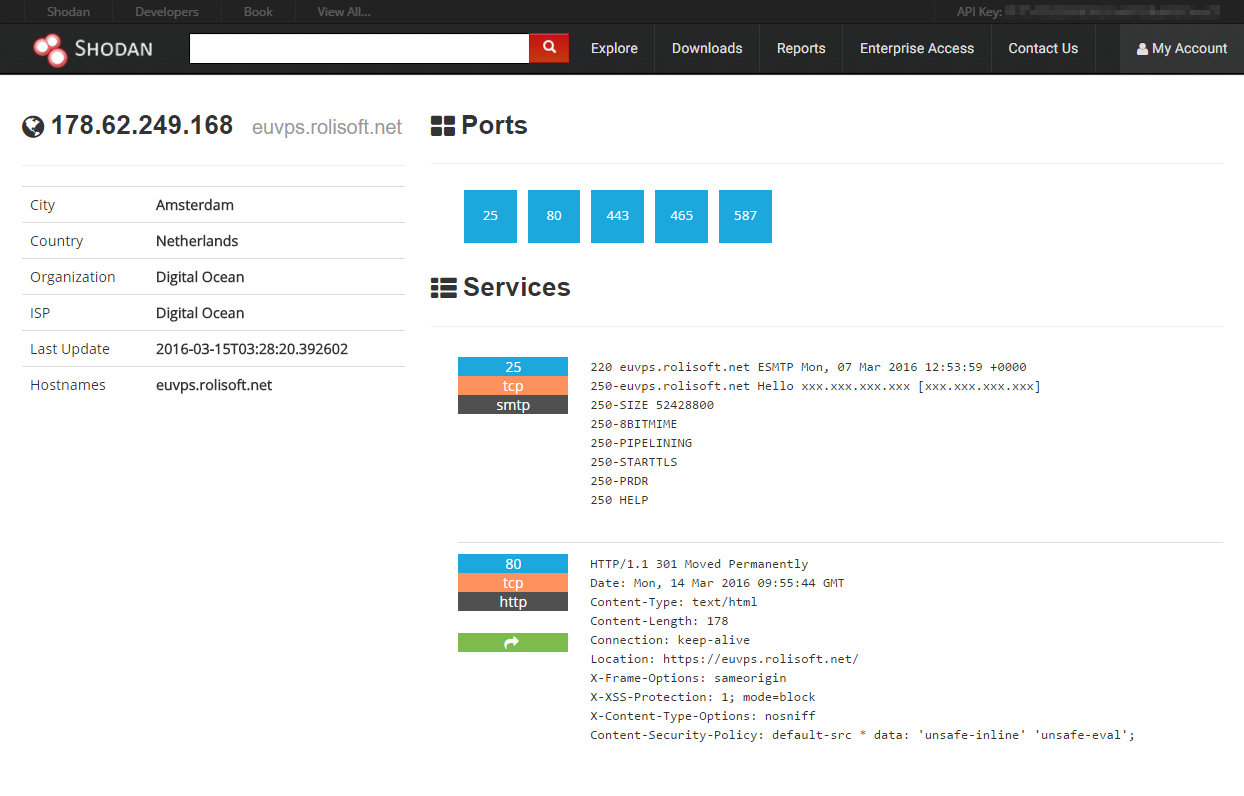
\includegraphics[scale=0.355]{shodan.png}
		\caption{178.62.249.168 adatai a Shodan-en}
		\label{shodanscr}
	\end{figure}
	
	Ahhoz, hogy az alkalmazásban Shodan adatot lehessen szerezni és felhasználni, a felhasználónak regisztrálnia kell egy ingyenes fiókot a \url{https://shodan.io/} címen, és az ott található API kulcsot specifikálnia kell az alkalmazásnak a \mintinline{bash}{--shodan-key} parancssori argumenton keresztül.
	
	Kivitelezési szempontból, a \mintinline{cpp}{ShodanScanner} komponens kommunikál a Shodan JSON API interfészével, és lekéri a kívánt IP címek adatait. Ezen komponens a \mintinline{cpp}{HostScanner} osztályból származik és emiatt az osztály helyettesíthet bármilyen más letapogató komponenst a szoftveren belül.

\subsubsection{Censys} \label{ssec:censys}

	A Censys\cite{censys15} egy Michigani Egyetem Régensei által készített és karbantartott szolgáltatás. Hasonlóan az előző szolgáltatáshoz, az adatait Internet-szerti letapogatási műveletek során gyűjti. Az adatokhoz fejlesztők és biztonsági kutatók hozzáférhetnek strukturált lekérdezések folyamán a projekt webes felületén vagy a REST API-ján keresztül. A \ref{censysscr}-as ábra bemutat egy példa lekérdezést a rendszertől egy bizonyos IP címre.
	
	\begin{figure}[!htbp]
		\centering
		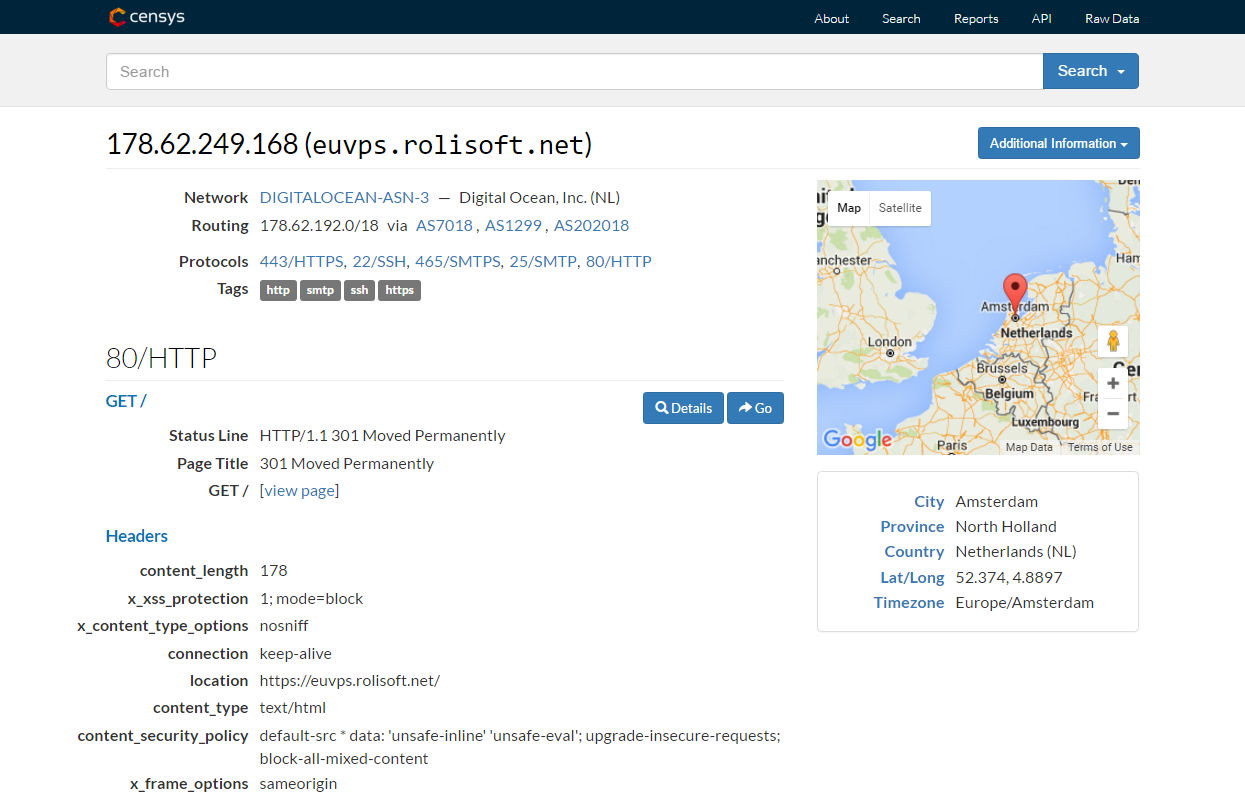
\includegraphics[scale=0.355]{censys.png}
		\caption{178.62.249.168 adatai a Censys-en}
		\label{censysscr}
	\end{figure}
	
	A projekt által használt letapogató szoftver, név szerint ZMap\cite{zmap13}, és a különböző komponensei nyílt-forrásúak. A letapogató által generált nyers adatok egy Internet-szerti letapogatás során is letölthetőek a Censys weboldalán bárki által és szabadon felhasználhatóak.
	
	Ahhoz, hogy az alkalmazásban Censys adatot lehessen szerezni és felhasználni, a felhasználónak regisztrálnia kell egy ingyenes fiókot a \url{https://censys.io/} címen, és az ott található UID és titkos kulcsot specifikálnia kell az alkalmazásnak a \mintinline{bash}{--censys-key} parancssori argumenton keresztül.
	
	Kivitelezési szempontból, a \mintinline{cpp}{CensysScanner} komponens kommunikál a Censys JSON API interfészével, és lekéri a kívánt IP címek adatait. Hasonlóan, ezen komponens is a \mintinline{cpp}{HostScanner} osztályból származik és emiatt az osztály helyettesíthet bármilyen más letapogató komponenst a szoftveren belül.

\subsubsection{Egyesítés}

	A \mintinline{cpp}{PassiveScanner} komponense az alkalmazásnak kérést kezdeményez a Shodan-en[\ref{ssec:shodan}] és a  Censys-en[\ref{ssec:censys}] egyiránt, majd az eredményeket egybevonja a végén.
	
	Az alkalmazás fejlesztési fázisa során az lett felfedezve, hogy általában mindkét szolgáltatásnak volt valamilyen információja egy bizonyos IP címről, viszont egyes esetekben az egyik szolgáltatásnak több információja volt, mint a másiknak, mélyebb elemzést sikerült végeznie, vagy csak egyszerűen hasznosabb volt a tárolt információ, mint a konkurensénél.
	
	Egy egész pontos példa az lenne, amikor egy IP cím esetén az egyik szolgáltatás valamilyen módon be lett azonosítva és ki lett tiltva a terheléskiegyenlítő által, mint ahogy ezt a \ref{shodanban}-es kódrészlet is mutatja, viszont a másik szolgáltatás sikeresen átjárt a terheléskiegyenlítőn és hasznos információt sikerült tárolnia a szolgáltatásról, mint ahogy ezt a \ref{censysnoban}-as kódrészlet is mutatja.
	
	\begin{listing}[H]
		\begin{minted}[style=pastie]{http}
			HTTP/1.1 403 You are banned from this site.  Please contact via a different client configuration if you believe that this is a mistake.
			Content-Type: text/html; charset=utf-8
			Date: Wed, 16 Mar 2016 01:17:18 GMT
			Retry-After: 5
			Server: Varnish
			X-Varnish: 2115087
			Content-Length: 590
			Connection: keep-alive
		\end{minted}
		\caption{54.193.103.xyz válasza Shodan számára egy tiltási hibaüzenettel}
		\label{shodanban}
	\end{listing}
		
	\begin{listing}[H]
		\begin{minted}[style=pastie]{http}
			HTTP/1.1 200 OK
			Content-Length: 3770
			Vary: Accept-Encoding
			Server: nginx/1.8.0
			Connection: keep-alive
			Last-Modified: Fri, 28 Aug 2015 19:43:39 GMT
			Content-Type: text/html
			Accept-Ranges: bytes
		\end{minted}
		\vspace{-5pt}
		\begin{minted}[style=borland,firstnumber=9]{html}
			 
			<!DOCTYPE html PUBLIC "-//W3C//DTD XHTML 1.1//EN" "http://www.w3.org/TR/xhtml11/DTD/xhtml11.dtd">
			<html xmlns="http://www.w3.org/1999/xhtml" xml:lang="en">
			<head>
			<!-- válasz többi része kivágva -->
		\end{minted}
		\caption{54.193.103.xyz válasza Censys számára tiltási hibaüzenet nélkül}
		\label{censysnoban}
	\end{listing}
	
	Fontos lenne itt megjegyezni, hogy a tiltott félnek küldött üzenet a \ref{shodanban}-es kódrészletben nem fedi fel a HTTP szerver nevét és verziószámát, míg a tiltatlan fél a \ref{censysnoban}-as kódrészletben a terheléskiegyenlítőn keresztül az élszerverhez kerül, és kiderül a szoftver neve illetve verziószáma, azaz ``nginx 1.8.0,'' amely épp tartalmaz egy \textbf{ismert távolról-kihasználható sebezhetőséget}\cite{nginxcve}.
	
	Azon esetekben, amikor mindkét szolgáltatás visszatérít egy szolgáltatási sávot egy bizonyos portnak, a hosszabb sáv lesz kiválasztva az egybevonási folyamat során. Ez a döntés azért volt meghozva így, mivel a tiltóüzenetek általában rövidebbek\cite{qualys11} a szolgáltatásmegtagadási támadások elkerülése végett, illetve az is lehetséges ilyenkor, hogy a hosszabb szolgáltatási sávon a szolgáltatás mélyebb elemzést is végzett (mint például a 'STARTTLS' parancs SMTP szervereknek a Censys által, de nem a Shodan által) amely azt jelenti, hogy a minta-alapú beazonosító komponensnek (a \ref{ssec:patternmatch}-s fejezetben tárgyalva) több bemeneti adat lesz elérhető.

\subsection{Külső Feltérképezés}

	Ez a fejezet bemutatja az alkalmazás \mintinline{cpp}{NmapScanner} komponensét, amely egy külső alkalmazást indít el a kért portok letapogatása érdekében, majd a külső alkalmazás által generált eredményeket beolvassa további elemzési célokból a jelenlegi alkalmazásba.
	
	Habár az alkalmazás tág körű letapogató komponenseket implementál, amint ezek tárgyalva vannak az \ref{ssec:icmpping}-es fejezettől az \ref{ssec:udpscan}-es fejezetig, egyesített interfésszel amely engedélyezi a feladatok könnyű és hatékony párhuzamosítását, redundanciaként a felhasználóknak fel van ajánlva az a lehetőség is, hogy egy külső alkalmazást használjanak a letapogatási célokra.
	
	A komponens, amint a neve is sugallja, az \textit{nmap} alkalmazást támogatja, viszont bármilyen más alkalmazás is használható amely nmap-kompatibilis XML-alapú jelentéseket képes generálni. Egy ilyen alternatív alkalmazásra példa a \textit{masscan} nevű szoftver lenne.
	
	Ahhoz, hogy az nmap-et használni lehessen letapogatásra, az \mintinline{batch}{nmap} alkalmazás elérhető kell legyen a \mintinline{batch} környezeti változón belül.
	
\subsection{Szerverek Minta-alapú Beazonosítása} \label{ssec:patternmatch}

	A \mintinline{cpp}{ServiceRegexMatcher} komponens feladata, hogy bemenetként fogadja a teljes szolgáltatási sávot, és futtassa le egy adatbázis ellen, amely reguláris kifejezéseket tartalmaz CPE nevekhez társítva.

	\begin{listing}[H]
		\begin{minted}{matlab}
			^HTTP/1\.[01] \d{3}.*\r\nServer: nginx(?:/([\d.]+))?
		\end{minted}
		\caption{Példa reguláris kifejezés \mintinline{matlab}{cpe:/a:nginx:nginx} szoftverhez}
		\label{nginxregex}
	\end{listing}
	
	A \ref{nginxregex}-es kódrészletben található reguláris kifejezés illeszkedik az ``nginx'' HTTP szoftver által generált válaszfejlécekre. Továbbá, a reguláris kifejezés tartalmaz egy opcionális csoportot, amely a verziószámot próbálja megkeresni. Amennyiben a kifejezés illeszkedik, a komponens visszatéríti a \mintinline{matlab}{cpe:/a:nginx:nginx:1.9.12} nevet, míg ha a kifejezés parciálisan illeszkedik, azaz a verziószám csoport nélkül, a \mintinline{matlab}{cpe:/a:nginx:nginx} név lesz visszatérítve.
	
	Ez különbözik a \ref{ssec:matchcpe}-s fejezetben leírt módszertől, ugyanis itt az azonosítás sikeres verziószám nélkül is, így a jövőbeli verziószámok is könnyen felismerhetőek a letapogató szoftver frissítése nélkül.
	
\subsubsection{Identitás Kikövetkeztetése Névhírdetés Nélkül}
	
	Míg a \ref{nginxregex}-es kódrészletben bemutatott kifejezés elég egyszerű, a minta alapú beazonosító komponenssel olyan szervereket is be lehet azonosítani, amelyek nem hirdetik ki a nevüket a szolgáltatási sávban.
	
	\begin{listing}[H]
		\begin{minted}{matlab}
			^554 SMTP synchronization error\r\n
		\end{minted}
		\caption{Példa reguláris kifejezés \mintinline{matlab}{cpe:/a:exim:exim} szoftverhez}
		\label{eximregex}
	\end{listing}
	
	A \ref{eximregex}-es kódrészletben bemutatott reguláris kifejezés az ``exim'' SMTP szerver szoftvert képes beazonosítani, ugyanis az 554-es hibakód standard, az ``SMTP synchronization error'' üzenet bájtról bájtra implementáció-specifikus, és különbözik más SMTP szoftverekben.
	
	Hasonlóan, a verziószámot is ki lehet következtetni bizonyos esetekben, ha tudjuk hogy milyen publikus üzenetek változtak a szerver szoftverben egyik verzióról a másikra, és ennek tesztelésére egy reguláris kifejezést írunk. (Például az `PRDR' támogatás megléte a szolgáltatási sávban, amely arra utal, hogy az exim szerver legalább 4.83-as verziójával van dolgunk, ugyanis ez az első verzió amelyben ez implementálva és kihirdetve van.)

\subsection{Szerverek CPE-alapú Beazonosítása} \label{ssec:matchcpe}

	A \textit{National Institute of Standards and Technology} karban tart egy \textit{National Vulnerability Database} nevű adatbázist, amely tartalmazza a publikusan elismert sebezhetőségek listáját a népszerűbb szoftvereknek. Ebben a fejezetben bemutatott komponens, a \mintinline{cpp}{CpeDictionaryMatcher} felhasználja ezen intézet által szabadon közzétett és naponta frissített \textit{Common Platform Enumeration Dictionary} listáját.
	
	A \textit{CPE} egy elnevezési rendszer hardver, szoftver illetve operációs rendszerek számára\cite{cpe22}. A 2.2-es formátumja: \mintinline{matlab}{cpe:/típus:tulajdonos:termék:verzió:frissítés:kiadás:nyelv} ahol a 'típus' komponens lehet \mintinline{matlab}{h} mint `hardver', \mintinline{matlab}{o} mint `operációs rendszer' és \mintinline{matlab}{a} mint `alkalmazás'.
	
	Példaként, az ``nginx 1.3.9'' CPE neve \mintinline{matlab}{cpe:/a:igor_sysoev:nginx:1.3.9}.
	
	Az előzőleg megemlített \textit{CPE szótár} egy gyűjteménye azon CPE neveknek, amelyekhez publikusan ismert sebezhetőség van csatolva a \textit{CVE adatbázisban}.
	
	Sajnos a CPE nevek nincsenek a szolgáltatási sávban feltüntetve, és nem létezik egy jól definiált módszer arra, hogy a szolgáltatási sávok alapján megkeressük a hozzátartozó CPE neveket. A \cite{shovat15} cikkben a szerzők hasonló problémát tárgyaltak, és az általuk bemutatott módszeren alapszik az alkalmazásban implementált CPE-alapú beazonosító komponens is.
	
\subsubsection{Kivitelezés Áttekintése}
	
	A jelenlegi CPE azonosító komponens memóriába tölti a teljes CPE szótár egy előre feldolgozott változatát, amelyben a CPE nevek tokenizálva vannak és a felesleges információ el van hanyagolva memóriahatékonysági okok miatt. A \ref{ciscotokens}-es kódrészlet bemutatja a memóriába betöltött struktúrát egy példa CPE névnek.
	
	\begin{listing}[H]
		\begin{minted}[style=perldoc]{js}
			CpeEntry {
				// cpe:/o:cisco:ios
				"ProductSpecificTokens": ["cisco", "ios"],
				"Versions": [
					CpeVersionEntry {
						// cpe:/o:cisco:ios:12.2sxi
						"VersionNumber": "12.2",
						"VersionSpecificTokens": ["sxi"]
					},
					CpeVersionEntry {
						// cpe:/o:cisco:ios:12.2sxh
						"VersionNumber": "12.2",
						"VersionSpecificTokens": ["sxh"]
					}
					// [további verziók kivágva]
				]
			}
		\end{minted}
		\caption{Megközelítő belső reprezentációja a \mintinline{matlab}{cpe:/o:cisco:ios:12.2sxi} bejegyzésnek}
		\label{ciscotokens}
	\end{listing}
	
	A tokenizációs folyamat során, a CPE név `tulajdonos' és `termék' komponenseit a \mintinline{matlab}{([a-z][a-z0-9]+)} reguláris kifejezés ellen van illesztve azon okból fogva, hogy azokat a szavakat amelyek több mint egy karakter hosszúak és nem számmal kezdődnek, egy külön token listába legyenek helyezve.
	
	Így példaként, a \mintinline{matlab}{cpe:/a:apache:tomcat:4.1.36} CPE név alapján készül egy tömb, amely a \mintinline[style=vs]{js}{["apache", "tomcat"]} tokeneket tartalmazza.
	
	A CPE verzió komponense bizonyos esetekben tartalmaz elhanyagolható karaktereket vagy non-standard verzió jelölést. Ezen esetek kiküszöbölése végett, a verziószám a \mintinline{matlab}{\d+\.(?:\d+\.)*\d+} reguláris kifejezés ellen van illesztve, amelynek szükséges legalább egy ponttal elválasztott két szám.
	
	Amennyiben a verzió komponens tartalmaz ezenkívül szavakat, ezek az első tokenizációs lépésben bemutatott reguláris kifejezés ellen vannak illesztve, és egy verzió-specifikus token tömbbe tárolva. Példaként ilyen esetekben, a \mintinline{matlab}{cpe:/o:cisco:ios:12.2sxi} CPE név esetén, a verzió-specifikus tokenek tömb tartalma \mintinline[style=vs]{js}{["sxi"]} lesz.
	
	CPE-alapú azonosítás során, a teljes adatbázis átiterálódik, először a termék-specifikus tokeneket próbálva. Amennyiben az összes token megtalálható a bemeneti szövegben, a termékhez csatolt verziószámok vannak kipróbálva. Amennyiben legalább egy verziószám talált, és van neki egy verzió-specifikus token tömbje is, az összes ilyen további tokennek is találnia kell.
	
\subsubsection{Élesetek Kezelése} \label{ssec:cpeedges}

	A \textit{Sun Microsystems} cég azonosító komponense a ``sun'', amely olyan CPE neveket eredményez, mint \mintinline{matlab}{cpe:/a:sun:jre}, \mintinline{matlab}{cpe:/a:sun:jdk} és \mintinline{matlab}{cpe:/o:sun:solaris:10.0}. A problémás része ennek a tokennek, hogy a legtöbb protokoll, mint például az SMTP és HTTP, visszatérítik a dátumot a szolgáltatási sávukban RFC 1123 formátumban\cite{rfc2616}, amely így néz ki: ``Sun, 14 Mar 2016 16:33:02 GMT''.
	
	A dátum első szava a nap neve, amely három betűre van rövidítve, és vasárnaponként az értéke ``Sun''. Ez bevezet egy bizonyos `véletlenszerűségi' alkotórészt a szoftverbe, ugyanis a pontozási rendszere a CPE alapú azonosítónak minden vasárnap nagyobb pontszámot fog társítani a \textit{Sun Microsystems} általi termékeknek, ugyanis a ``sun'' token immáron megtalálható az elemzett szolgáltatási sávban.
	
	\begin{listing}[H]
		\begin{minted}{matlab}
			Cisco IOS Software, s72033_rp Software (s72033_rp-IPSERVICESK9_WAN-M), Version 12.2(33)SXI3, RELEASE SOFTWARE (fc2)
			Technical Support: http://www.cisco.com/techsupport
			Copyright (c) 1986-2009 by Cisco Systems, Inc.
			Compiled Tue 27-Oct-09 11:12 by prod_
		\end{minted}
		\caption{Példa telnet szolgáltatási sávja bizonyos Cisco routereknek}
		\label{ciscosvcbnr}
	\end{listing}

	Egy másik problémás példa a Cisco verziójelölése lenne a saját telnet szolgáltatásuk sávjában. A \ref{ciscosvcbnr}-es kódrészletben bemutatott szolgáltatási sáv a \mintinline{matlab}{cpe:/o:cisco:ios:12.2sxi3} CPE névhez tartozik. A probléma onnan adódik, hogy Cisco a $12.2$-es verziószámmal és ``sxi'' frissítési szint mellett ``by'' frissítési szintet is publikált: \mintinline{matlab}{cpe:/o:cisco:ios:12.2by}.
	
	Ha a két CPE nevet tokenizálnánk, a két különböző token tömb úgy nézne ki, hogy \mintinline[style=vs]{js}{["cisco", "ios", "sxi"]} és \mintinline[style=vs]{js}{["cisco", "ios", "by"]}. A verziószám és az első két token mindkét tömbből találna, viszont a harmadik tokenek ``sxi'' és ``by'', mindkét tömbből ugyancsak találnának. A harmadik és negyedik sorában a \ref{ciscosvcbnr}-es kódrészletnek a ``copyright'' és ``compiled'' sorok mindketten tartalmazzák a ``by'' szavat.

	Az előzőleg említett ShoVAT\cite{shovat15} cikk úgy oldotta meg ezt a problémát, hogy azon tokeneket amelyek közelebb vannak a verziószámhoz nagyobb súllyal látta el, mint azokat, amelyek messzebb vannak. Ezen dolgozat céljából fejlesztett alkalmazás is ezt a módszert alkalmazza a helyes CPE név kiválasztására hasonló helyzetekben.
	
	\begin{multicols}{2}
		\begin{listing}[H]
			\begin{minted}[style=pastie]{http}
				HTTP/1.1 200 OK
				Server: nginx/1.9.12 (Ubuntu)
				X-Powered-By: PHP/5.6.19
				Date: Fri, 11 Mar 2016 16:04:07 GMT
				Connection: close
			\end{minted}
			\caption{Példa HTTP válasz}
			\label{httpsvcbnr}
		\end{listing}
		\begin{listing}[H]
			\begin{minted}[style=perldoc]{js}
				[
					"nginx/1.9.12",
					"Ubuntu",
					"PHP/5.6.19"
				]
			\end{minted}
			\caption{Kiszűrt tokenek a példából}
			\label{httpsvcbnrtokens}
		\end{listing}
	\end{multicols}
	
	Egy alternatív módszer van bemutatva a \ref{httpsvcbnr}-as illetve \ref{httpsvcbnrtokens}-es kódrészletekben, amelyet a szoftver még alkalmaz redundanciaként az az, hogy olyan protokollok esetén ahol ismert a szervernév kihirdetésének helye (mint például 'Server' és `X-Powered-By' mezők HTTP esetén) ott csak ezek a mezők ellen lesz lefuttatva a CPE azonosító, míg azon protokollok esetén ahol nincs standard hely a szervernév kihirdetésére (mint például SMTP) ott megpróbál minél több haszontalan információt (mint például hibaüzenetek, hoszt név vagy dátumok) kivágni az álpozitív találatok kiszűrése érdekében.

\newpage
\section{Bibliográfia}

	\begingroup
	\renewcommand{\section}[2]{}
	\renewcommand{\markboth}[2]{}
		\bibliography{thesis}
		\bibliographystyle{thesis}
	\endgroup

\end{document}